\documentclass[tikz,border=6pt]{standalone}
\usepackage{xcolor}
\begin{document}
% Canonical ch-diagram for 2_1^-1
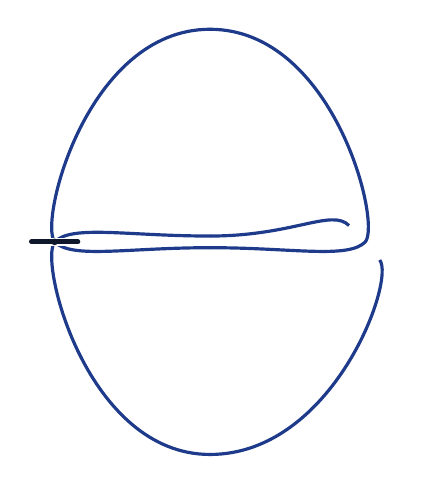
\begin{tikzpicture}[line join=round]
  \definecolor{skcomp0}{RGB}{30,58,138}
  \definecolor{skmark}{RGB}{15,23,42}
  \draw[skcomp0, line width=1.15pt, line cap=butt] (2.1085,-0.2302) .. controls (2.3132,-0.4891) and (1.5122,-2.7000) .. (-0.0466,-2.7000);
  \draw[skcomp0, line width=1.15pt, line cap=butt] (1.7192,0.2075) .. controls (1.4987,0.4279) and (1.0128,0.0740) .. (-0.0466,0.0740);
  \draw[skcomp0, line width=1.15pt, line cap=round] (-2.0198,-0.0000) .. controls (-2.2245,0.2589) and (-1.6055,2.7000) .. (-0.0466,2.7000);
  \draw[skcomp0, line width=1.15pt, line cap=round] (1.9266,-0.0000) .. controls (2.1313,0.2589) and (1.5122,2.7000) .. (-0.0466,2.7000);
  \draw[skcomp0, line width=1.15pt, line cap=round] (-2.0198,-0.0000) .. controls (-2.2245,-0.2589) and (-1.6055,-2.7000) .. (-0.0466,-2.7000);
  \draw[skcomp0, line width=1.15pt, line cap=round] (-2.0198,-0.0000) .. controls (-1.7994,-0.2204) and (-1.1060,-0.0740) .. (-0.0466,-0.0740);
  \draw[skcomp0, line width=1.15pt, line cap=round] (1.9266,-0.0000) .. controls (1.7062,-0.2204) and (1.0128,-0.0740) .. (-0.0466,-0.0740);
  \draw[skcomp0, line width=1.15pt, line cap=round] (-2.0198,-0.0000) .. controls (-1.7994,0.2204) and (-1.1060,0.0740) .. (-0.0466,0.0740);
  \draw[white, line width=2.8pt, line cap=round] (-2.3132,-0.0000) -- (-1.7265,-0.0000);
  \draw[skmark, line width=1.85pt, line cap=round] (-2.3132,-0.0000) -- (-1.7265,-0.0000);
  \fill[skmark] (-2.0198,-0.0000) circle (1.2pt);
\end{tikzpicture}
\end{document}
